%% LyX 2.0.0 created this file.  For more info, see http://www.lyx.org/.
%% Do not edit unless you really know what you are doing.
\documentclass[english]{article}
\usepackage[T1]{fontenc}
\usepackage[latin9]{inputenc}
\usepackage{array}
\usepackage{multirow}
\usepackage{graphicx}

\makeatletter

%%%%%%%%%%%%%%%%%%%%%%%%%%%%%% LyX specific LaTeX commands.
%% Because html converters don't know tabularnewline
\providecommand{\tabularnewline}{\\}
%% A simple dot to overcome graphicx limitations
\newcommand{\lyxdot}{.}


%%%%%%%%%%%%%%%%%%%%%%%%%%%%%% Textclass specific LaTeX commands.
\newenvironment{lyxlist}[1]
{\begin{list}{}
{\settowidth{\labelwidth}{#1}
 \setlength{\leftmargin}{\labelwidth}
 \addtolength{\leftmargin}{\labelsep}
 \renewcommand{\makelabel}[1]{##1\hfil}}}
{\end{list}}

%%%%%%%%%%%%%%%%%%%%%%%%%%%%%% User specified LaTeX commands.




\usepackage{babel}

\makeatother

\usepackage{babel}
\begin{document}

\title{Performance Report on EC2 Instances}


\author{Vineet Kumar, Phuc Xuan Nguyen}

\maketitle

\section{Introduction}

Amazon Elastic Compute Cloud(EC2) is a web service that provides resizable
computing power through the cloud. There are lots of disputes online
regarding the correctness of the {}``rated'' hardware performance
of Amazon EC2. Some articles claims that the actual performance of
the hardware is much less than the advertised number. We are interested
in testing to see whether such claim is accurate, and if not, what
the reason might be. As a later part of the project, we are also interested
in the overhead of the linux containers(LXC) on a virtualized platform.

The aim of this project is to measure performance on Amazon's EC2
instances. For the first portion of this project we measure the overhead
of CPU, scheduling and OS services. All the code for our tests was
written in C. We used gcc 4.6.1 with no optimizations to run our code.
Machine description, measuring procedure call overhead, measuring
memory latency, RAM bandwidth and networking experiments were done
by Phuc Xuan Nguyen. Rest of the measurements were done by Vineet
Kumar. I think we spent a total of 20 working days on the project.


\section{Machine Description}

We are aiming to measure the performance on the Amazon's t1.micro
instances. 
\begin{itemize}
\item 1 Elastic Computing Unit 
\item Processor: Intel(c) Xeon(R) CPU E5430 @ 2.66Ghz.

\begin{itemize}
\item 12M L2 Cache, 1333 Mhz FSB 
\end{itemize}
\item Memory: 592MiB 
\item Netword card speed

\begin{itemize}
\item Between EC2 Instances: 100MB/s 
\end{itemize}
\item Disk: Amazon Elastic Block (EBS)

\begin{itemize}
\item Size: 7.9GB 
\end{itemize}
\item Operating System: Ubuntu Oneric 11.10 
\end{itemize}

\section{CPU Operation}

For all our experiments we use RDTSC counter. To obtain time we divide
this by the CPU frequency. Also of all the data seen, we discard the
best and worst 10\% of data and then take mean values.


\subsection{Measurement overhead}


\subsubsection{Experiment}

We are using RDTSC as a fine-grained counter to measure the performance.
In order to calculate the overhead of RDSTC, we run the following
experiment.

Function 1: 
\begin{itemize}
\item Get initial clock counter 
\item Repeat N times:

\begin{itemize}
\item Run RDTSC 
\item Perform a random function f 
\end{itemize}
\item Return the difference between the current and the initial clock counter. 
\end{itemize}
Function 2: 
\begin{itemize}
\item Get initial clock counter 
\item Repeat N times:

\begin{itemize}
\item Perform a random function f 
\end{itemize}
\item Return the difference between the current and the initial clock counter 
\end{itemize}
To measure the for loop overhead, we set up two procedures: (1) using
a for loop to execute a function foo() N times, and (2) (baseline)
just execute foo() N times in a row. N is a random number generated
uniformly from 100-1000. Through experiment we find that the amount
of times does not affect the interested results.


\subsubsection{Prediction}

In this experiment, we would expect that Function 2 will yield higher
clock cycles than than Function 1 due to the overhead of RDTSC. Since
these are simple function, the overhead will be significany compared
to the overall running time.

For for-loop overhead prediction, we expect at least 6 clocks cycles
will be added on to the baseline performance due to the facts that
the for-loop must be recompiled into different read word, set word
instructions. For example, for(int x = 0; x < N; x++) would incur
the cost for set x to be 0, the branch to check if x less than N,
and a read word and set word for x++. These are not accounted for
the branch overhead caused by the for loop logic itself.


\subsubsection{Results}

We find that the variance becomes insignificant when N is around 10000.
We avoid the possible compiler optimization by running the random
function f.

We calculate the difference in the result of Function 2 and Function
1 and divide that by N to find the overhead of RDTSC. In the t1.micro
instance. 
\begin{itemize}
\item Without RDTSC: average 6.00 cycles \textasciitilde{} 2.25 $\mu s$ 
\item With RDTSC: average 48 cycles \textasciitilde{} 18.04 $\mu s$ 
\item The overhead of RDSTC: \textasciitilde{} 15.789$\mu s$ 
\end{itemize}
After running the for-loop experiment 10000 times, we find that 
\begin{itemize}
\item Without for loop: average 12.6 cycles \textasciitilde{} $4.7\mu s$ 
\item With for loop: average 21.8 cycles \textasciitilde{} $7.89\mu s$ 
\end{itemize}
So the overhead of the for loop is the difference between these, which
is 9.2 cycles \textasciitilde{} $3.38\mu s$.


\subsubsection{Dicussion}

The result is as expected. Function 2 yields an extra 42 cycles as
the overhead for RDSTC. Our for loop estimations falls on the short
side as the number of extra cycles is 9.2 cycles instead of 6 as predicted.

We notice that these overhead is significant in our experiment, 700\%
for RDTSC and 75\% for for-loop. However, these are simple experiment,
where the running time order stays around single or double digits
of microseconds. Later experiment will show the other software overhead
would result much higher overhead than these measurement overhead.


\subsection{Procedure call overhead}

To find out the procedure call overhead, we perform two simple operations
(int x = 1+1; int y = x;) in 9 different scenarios: no procedure call
and procedure calls with the 0-7 parameters.


\subsubsection{Prediction}

We expect a roughly linear increase in the clock cycles as the number
of parameters increase. The reason of linearity is that we have no
reason to doubt any other factors could contribute to the increase
in clock cycle besides the time to copy the value into the parameter


\subsubsection{Results}

The result, gathered after running 1,000,000 iterations, is shown
in Figure 1.

\begin{figure}
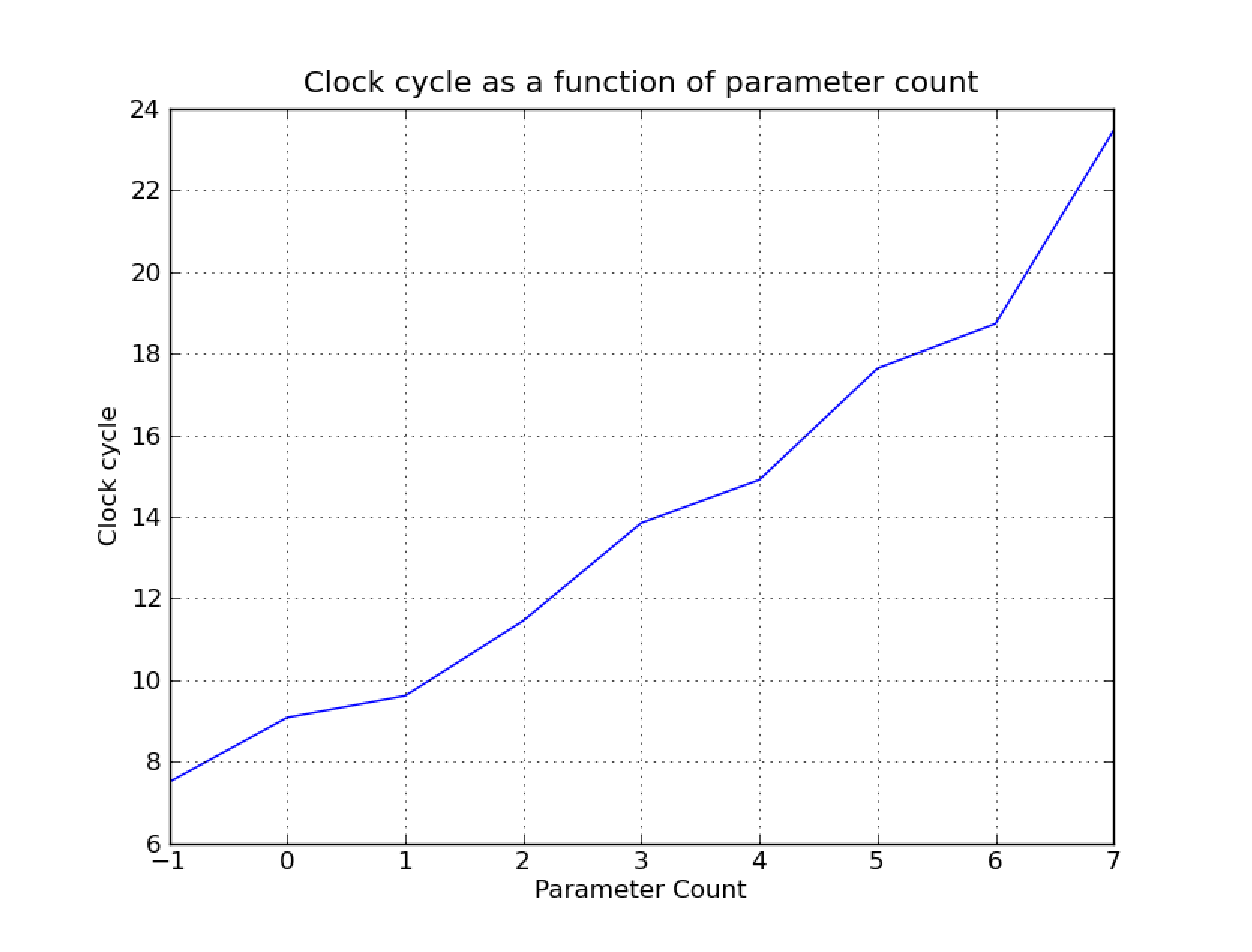
\includegraphics[scale=0.5]{procedure_call_result}

\caption{Procedure call as a function of paramter count}
\end{figure}



\subsubsection{Discussion}

The result shows a roughly linear increase in the clock cycles, as
predicted.


\subsection{System call overhead}
\begin{enumerate}
\item Prediction - System Call is a slightly heavier call than a simple
procedure call, it needs to do more checks and in effect is the only
domain crossing for our system. Thus we predict that system call overhead
time would be little more than a procedure call. Its hard to make
other predictions for a system call. 
\item Experiment: To measure system call overhead, we need to do measurements
on a system call that does not do much work. We do our experiments
by calling {}``getpid()'' and by writing one byte to the device
devnull. We notice that for both these experiments if we run a tight
loop within a single process, the system call gets cached and thus
does not give us correct overhead measurements. Thus, we handle this
issue by running the test within a context of different process. We
run the test for 10,000 iterations. Table 1 shows the results:Results:
The following table shows the results: 
\item Results : 
\end{enumerate}
Table 1: System call overhead

\begin{tabular}{|l|c|c|c|c|}
\hline 
System Call  & Time - cached($\mu$s)  & Std. dev & Time - uncached($\mu$s)  & Std. dev\tabularnewline
\hline 
\hline 
getpid()  & 0.00358 (9.66 M cycles)  & 1.71$\%$  & 7.89 (21303 M cycles)  & 5.74\%\tabularnewline
\hline 
write to devnull  & 0.00341 (9.21 M cycles)  & 1.06\%  & 1.45 (3915 M cycles)  & 53\%\tabularnewline
\hline 
\end{tabular}
\begin{enumerate}
\item Analysis : We see that the time needed for a getpid() is slightly
more than a procedure call 
\end{enumerate}

\subsection{Task creation time}

Prediction : We epect task creation to take much more time than a
system call, as it involves context switch when a new task needs to
created. We expect kernel thread creation to take less time as in
effect a user thread is tied to kernel.

We measure the task creation time by calling the timer before a fork()
is issued and immediately inside the child process. We repeat this
process for 10, 000 iterations. To measure the creation time for a
kernel thread - we use posix thread attributes to tie a user thread
to a kernel level thread. We repeat these experiments 10,000 times.
We use the following test methodology : 
\begin{enumerate}
\item Repeat N times 
\item Start timer 
\item Fork a process 
\item Stop timer inside the child process 
\end{enumerate}
\begin{table}
Table 2: Process and kernel thread creation overhead

\begin{tabular}{|c|c|c|}
\hline 
 & Time($\mu$s)  & Std. deviation\tabularnewline
\hline 
\hline 
Process creation  & 264.73(714771 M cycles)  & 18.48\%\tabularnewline
\hline 
Kernel Thread Creation  & 1.89 (5103 M cycles)  & 35 \tabularnewline
\hline 
\end{tabular}
\end{table}


Analysis : Process creation time takes much longer than kernel thread
creation, a part of the explanation could be that process creation
needs to do domain crossing, whereas kernel thread creation does not.


\subsection{Context switching time}

Prediction : We expect context switch time to take atleast the time
needed for system call.

We measure context switch time by passing a token across pipes. We
create a total of 4 pipes to accomplish a 2 way communication and
measure the round trip time. This roundtrip time per process contains
time needed to conext switch twice and time for a read and write call
using pipes. We however, do not remove the pipe overhead - that needs
to be done. We run our experiments for N iterations

This is the test methodology we use for measuring a process context
switch time 
\begin{enumerate}
\item Create 2 pipes for communication between process 1 and process 2 (pipe1) 
\item Create 2 pipes for communication between process 2 and process 1 (pipe2) 
\item Repeat N times

\begin{enumerate}
\item Start timer 
\item Repeat (c) -(d) for some iterations 
\item Process 1 writes to pipe1, process 2 reads it. Note that these will
be blocking reads. This causes Process 2 to start running 
\item Process 2 writes to pipe2 and process 1 reads it. This will again
cause a context switch 
\item Stop timer 
\end{enumerate}
\end{enumerate}
For Measuring kernel thread context switch time we use posix threads
bound to kernel by setting scope attribute to PTHREAD\_SCOPE\_SYSTEM
\begin{table}
Table 3: Context Switching overhead

\begin{tabular}{|c|c|c|}
\hline 
 & Time ($\mu$s)  & Std. deviation\tabularnewline
\hline 
\hline 
Process Context Switch  & 2.19 (5913 M cycles)  & 27.8\%\tabularnewline
\hline 
Kernel thread context switch  & 2.65 (7155 M cycles)  & 38.5\%\tabularnewline
\hline 
\end{tabular}
\end{table}


Analysis : Table shows that context switch time is of the order of
a system call, and that kenrel thread conext switch does not vary
much with process context switch time.


\section{Memory}


\subsection{RAM Access Time}


\subsection{Experiment}

We are setting up a similar pointer-chase experiment as Bradley et.
al. We want to measure performance of repeated memory access to integer
arrays with various sizes.


\subsection{Prediction}

Based on our hardware, we predict the the number of cycles will be
relatively small(\textasciitilde{}5 cycles) for L1 cache hit. The
cycles will stay constant until the array size is close to the L1
cache size. The number cycles will increase at this point. The cycles
will remain fairly constant until the array size is close to the L2
cache size, but there will be bump as page replacement policy in Linux
is non-deterministic. After the L2 cache size, the number of cycles
will increase and flat out with the rate equal to the memory read
rate.

Since we don't expect Amazon's VM to pin the guest OSes to cores.
Some of the data points will have significant variation due to cache
contention with other guest OSes running on the same core. We still
hope to discover some trend regardless of this anomaly.


\subsection{Result}

Figure 1 describes the average number of cycle to read an individual
integer from an array with different size on our local machine with
the L1 cache of 2x32KB instruction caches and 2x32KB caches and the
L2 Cache of 1MB. The Y-axis describes the number of cycle. The X-axis
describes the size of the array.

Figure 2 describes the same content but on EC2 t1.micro instance.


\subsection{Discussion}

Figure 1 matches out prediction. On our local machine, we find that
the average number of cycles to access an individual integer in an
array stays constant at \textasciitilde{}9 cycles and increase at
the L1 cache size of 32KB. Since Linux use non-deterministic page
mapping policy, cache conflicts occur quite often after in the L2
cache. The number of cycles flat out at \textasciitilde{}96 cycles.

However, Figure 2 has many high spikes due to cache contention as
the Xen does not pin the guest OSes to cores. If we ignore these data
points. Figure 3 is the result of taking out the spike. From Figure
3, we can see that it averages at \textasciitilde{}10 cycles per read
for L1 cache and increase to \textasciitilde{}17 cycles around at
the array size of 16KB. The number of cycles to read an integer from
memory is \textasciitilde{}178 cycles.

We underestimated the number of cycles to read an individual integer
from an array. This can be due to system overhead.

\begin{figure}
\includegraphics[scale=0.25]{mem_latency_local}

\caption{Memory Latency on Local Machine}
\end{figure}


\begin{figure}
\includegraphics[scale=0.25]{mem_latency_ec2_unmodifed}

\caption{Memory Latency on EC2}
\end{figure}


\begin{figure}
\includegraphics[scale=0.3]{mem_latency_ec2_modifed}

\caption{Memory Latency on EC2, removed outliners}
\end{figure}



\subsection{RAM Bandwidth}
\begin{description}
\item [{{{a)}}}] Prediction - To Predict RAM Bandwidth we need to multiply
the memory bus size with the memory clock speed. Our bus size is 64
bits which is 8 bytes. And our memory clock speed is 800 MhZ - which
gives us a maximum theoretical transfer rate of 6.4 GB /s. We predict
that the write bandwidth would be less than this as it needs to handle
issue of page cache eviction 
\item [{{{b)}}}] Experiment for Read Bandwidth : \end{description}
\begin{itemize}
\item We create a large array in the memory 
\item In a tight unrolled for loop - we access array elements at interval
of L2 cache size and add them up. Since our loop is unrolled 4 times,
this operation should cause 8 memory read operations from DRAM to
L2 
\item We measure beforehand amount of data transfered between DRAM and L2
for accessing 4 bytes. We found this to be 4K. 
\item We stop the timer that was started before 8 memory read opertaions.
We would have read 32K in one loop iteration. We divide this by time
taken and get the memory bandwidth\end{itemize}
\begin{description}
\item [{{{c)}}}] Experiment for Write Bandwidth :\end{description}
\begin{itemize}
\item We create a large array in the memory 
\item In a tight unrolled for loop - We add 2 fixed integers and store the
result at an interval of L2 size in our array 
\item We stop the timer that was started before 8 memory write operations\end{itemize}
\begin{description}
\item [{{{d)}}}] Block Transfer:\end{description}
\begin{itemize}
\item We do a L2 size block transfer from one memory location to another
in a loop. We measure time it takes to do the transfer 
\item This transfer will involve one read and possibly 2 write operations.
Thus we expect the bandwidth seen by this operation as average of
read and write bandwidth \end{itemize}
\begin{description}
\item [{{{e)}}}] Results: 
\item [{{{%
\begin{tabular}{|c|c|c|c|}
\hline 
 & CPU Cycles  & Std. Deviation  & Bandwidth GB /s\tabularnewline
\hline 
\hline 
Read  & 41,518  & 0.05 \%  & 2.076\tabularnewline
\hline 
Write  & 98, 781  & 0.03\%  & 0.878\tabularnewline
\hline 
Block Transfer  & 49,223,872  & 0.023\%  & 1.279\tabularnewline
\hline 
\end{tabular}}}}] ~ 
\item [{{{f)}}}] Analysis:\end{description}
\begin{itemize}
\item Block tarnsfer test results macth up with what we expected. We expected
the bandwidth to be average of read and write bandwidth numbers 
\item However, out orginal estimation seems to be off by quite a lot. We
expected to see a bandwidth of 6GB /s and saw 2 GB / s - We can attribute
it to the fact that we are running it on top of hypervisor and thus
page fault time could take more time as PTEs need to be installed
in the hypervisor's shadow page tables. 
\end{itemize}

\subsection{Page Fault Service Time :}
\begin{description}
\item [{{{a)}}}] Prediction :- To estimate page fault service time
we wanted to measure raw time of reading a page from disk. This is
hard to do from user space - but we can measure tiem to read a file
without using page cache. This would still include an overhead of
copying data between buffers - so while making an estimate we should
note that this estimate at best would be upper bound on page fault
service time. \end{description}
\begin{itemize}
\item We measure the time to do a disk read by measuring cost of doing a
direct read using 'dd' and redirecting output to /dev/null 
\item We notice that this gives us a speed of 5.1 MB/s -> Note that this
is a gross underestimate - it includes time to copy data between buffers 
\item Based on the clock speed and bandwidth and page size - we estimate
that around 2.1 million cycles will be needed\end{itemize}
\begin{description}
\item [{{{b)}}}] Experiment :- Our aim is to measure the page fault
service time. This means we want to measure the time it takes to do
a major page fault. This includes the time needed to bring the page
from the disk. We use an mmap (followed by no read aheads) to measure
the same. This works as mmap does a on demand page fault. Page is
faulted in only on first access. Below is a detailed description of
our experiment :\end{description}
\begin{itemize}
\item Create a Large File ( > 1.5 G) using a simple dd tool 
\item Determine page size by calling 'getconf PAGESIZE' - This gives us
page size of 4096 bytes or 4K on our system 
\item Call a posix\_fadvise with flag FADVISE\_DONTNEED. We do this to make
sure that a page is always brought in from the disk and not cached.
This is equivalent of dropping the page cache (by calling echo 1 >
/proc/sys/vm/drop\_cache) 
\item Memory Map the file using 'mmap' system call with flags 'MAP\_PRIVATE'.
We do this as we just want to do a read on the file. 
\item Do a madvise on the memory mapped area using MADV\_RANDOM. Do tests
both with and without MADV\_RANDOM 
\item Start timer 
\item Access a random page by reading a page address. This will cause a
major page fault. 
\item End timer. Report the time between start and end of timer.\end{itemize}
\begin{description}
\item [{{{c)}}}] Results : The table below shows results for reading
one page (4096) . Column 1 and 2 show results without madvise and
Columns 3 and 4 show results with madvise 
\item [{{{%
\begin{tabular}{|c|c|c|c|}
\hline 
 & Avg. CPU Cycles  & Std. Deviation(CPU Cycles)  & Time\tabularnewline
\hline 
\hline 
Page Fault (w/o) madvise  & 58,578  & 0.7625\%  & 21ms\tabularnewline
\hline 
Page Fault (with) madvise  & 197,190  & 0.1898\%  & 73 ms\tabularnewline
\hline 
\end{tabular}}}}] ~ 
\item [{{{d)}}}] Analysis :-\end{description}
\begin{itemize}
\item Our estimate was 2.1 Million CPU Cycles and what we got was 0.2 Million
cycles. As explained above, our estimate had some overhead due to
copying of data between buffers. Thus we expected the actual time
to be smaller 
\item Its interesting to note that if we dont give an madvise 'advice' for
our memory map region, we get better numbers. But those numbers are
most likely incorrect. We think if we dont do madvise, we hit pages
in page cache and thus the fault time does not remain as major page
fault service rate. 
\item To conclude, to measure page fault service rate, we need to ensure
that the page is brough in by reading from disk 
\end{itemize}

\section{Networking}


\subsection{Round trip time}

Round trip time is defined as the transmission times between two points
of a signal. More specifically, it is defined as the time it takes
for a packet to be sent plus the time for the response to come back.


\subsubsection{Experiment setup}

In the effort to compare the result with the ping time, we make sure
that we are the same amount of bytes. In Unix's ping, the default
option is 84 bytes per ping. We know that the TCP header is 20 bytes,
we will pad 64 bytes on to the data, to create the same amount.

We set up two identical instances: one server and one client. Client
will boot up, acquire the connection with the server, and then send
him a 64 bytes message (84 bytes with TCP headers). Server will process
the message, copy it into its buffer and send it back to the client.
Client receives the messages, record statistics, and quit.


\subsubsection{Prediction}

To get an idea of the RTT time between the two EC2 instances, we ping
the server instance. Results from pinging yields the average of .444ms.
We predict that our experimental result will be less than the estimate
due to the fact that ICMP is handled in the kernel and TCP needs to
cross the protection boundary. In the CPU scheduling part, we reported
that the cost of the syscall is around


\subsubsection{Experimentation Results}

After 1000 data points, we come to the following statitics. Table
1 describes the round trip remote statistics. Table 2 describes the
round trip loopback statistics.

The following results obtained by the following command in Unix: \textbf{ping
-c 100 10.211.45.127}

--- 10.211.45.127 ping statistics ---

100 packets transmitted, 100 received, 0\% packet loss, time 98998ms

rtt min/avg/max/mdev = 0.356/0.590/11.939/1.154 ms

The following results obtained by the following command in Unix: \textbf{ping
localhost}

--- localhost.localdomain ping statistics ---

723 packets transmitted, 723 received, 0\% packet loss, time 722009ms

rtt min/avg/max/mdev = 0.020/0.033/0.094/0.005 ms

\begin{table}
\begin{centering}
\begin{tabular}{|c|c|c|c|c|}
\hline 
 & min  & max  & average  & std\tabularnewline
\hline 
\hline 
clock cycles  & 1867624  & 2417024  & 2066900  & 122720\tabularnewline
\hline 
time(ms)  & 0.718  & 0.9296  & 0.79  & 0.0472\tabularnewline
\hline 
\end{tabular}
\par\end{centering}

\caption{Round trip remote statistics}
\end{table}


\begin{table}
\begin{centering}
\begin{tabular}{|c|c|c|c|c|}
\hline 
 & min  & max  & average  & std\tabularnewline
\hline 
\hline 
clock cycles  & 738360  & 982656  & 793550  & 56771\tabularnewline
\hline 
time(ms)  & 0.2839  & 0.377  & 0.31  & 0.0218\tabularnewline
\hline 
\end{tabular}
\par\end{centering}

\caption{Round trip loopback device}
\end{table}



\subsubsection{Discussion}

The ping statistics for both remote and loopback device is better
than the round trip time. As mentioned, in our prediction, this could
mainly caused by the fact that ICMP is handled through the kernel
and TCP is handled in the user address space. The cost of context
switching and crossing address space adds up to the difference.

We also notice that ping time is an order of magnitude better than
round trip loopback device time. We attribute this fact to the possibility
that the ping call wouldn't leave the kernel space for the localhost
to copy the package data to the network card. As opposed to the round
trip, first we have to call send, which involves in a switch to the
kernel space. The data is then copied to the network card, and triggers
an interrupts to the user space.

The RTT time for the loopback device could be considered as the OS
software overhead, as packet is directly copied into the network card.
The baseline network performance would be the difference between the
loopback device RTT and the remote RTT. According to this logic, the
ideal RTT without the OS overhead would be (0.79-0.31) = .48ms. From
this result, we can see that the software overhead is 64.5\% of the
ideal situation. However, if we look at the ping performance, the
ideal RTT for ping is (0.590-0.033) = 0.577ms, the overhead to ideal
ratio is only 5.9\%. This experimentation shows that handling networking
protocol insides the kernel would have a great impact on the round
trip performance.


\subsection{Peak bandwidth}


\subsubsection{Experiment Setup}

We set up two identical instances: a server and a client. The client
will connect to the target server, and sending various amount of data
to the servers. The amount ranges from 1MB to 400MB.

Unlike the previous experiment, we are measuring the performance on
the server side. Server will wait for a connection and starts reading
from the the socket. After each read, it will record the running total
of bytes reading so far and the amount of clock cycles to read it.

We set the buffer window on the server size to be 20000 bytes. We
believe that this value is sufficient to make the overhead caused
by looping to be insignificant.


\subsubsection{Prediction}

To get an idea of the data transfer rate between two instances, we
perform a quick scp command between two instances to transfer a 1GB
files. We notice the TCP connection starts off with the data transfer
rate of 30MB/s. However, it quickly degrade to around 10MB/s. We also
see that the data transfer rate fluctuate very often. So, it is hard
to pin down the exact prediction of the average and peak bandwidth.
From the number from SCP experiment, we conjecture that the peak bandwdith
would be around 30MB/s and the average bandwidth would be around 15MB/s.


\subsubsection{Results}

Figure shows the bandwidth corresponding to the total data size sent
and Figure shows the same image for the loopback device.

\begin{figure}
\includegraphics[scale=0.25]{bandwidth}

\caption{Bandwidth for remote case vs. total data size transfer}
\end{figure}


\begin{figure}
\includegraphics[scale=0.25]{bandwidth\lyxdot loopback}

\caption{Bandwidth for loopback case vs. total data size transfer}
\end{figure}



\subsubsection{Discussion}

For the remote case, we get the peak bandwidth at 30MBps and a huge
drop-off after the 150MB point to around 10MBps. This is due to the
TCP implementation, where they would allow the connection proceeds
with a higher speed at first, then slowly takes away the bandwidth.
While the loopback decide maintains a fairly high bandwidth between
900MBps and 1.1Gbps

As the packet are delivered directly to the network card in the loopback
case, we can use the data for loopback device as the software overhead
of the network. In order to see what ideal performance of the network,
we look at the data points with the highest bandwidth and compare
the clock cycles from the same settings. For example, we look at the
data point where data size is 100MB, the difference in clock cycles
to transmit that data is (8309437712 - 232012888) = 8077424824 cycles.
So the OS overhead is extremely small in this case, 2\% of the ideal.
The slowdown in bandwidth is mostly due to network transaction.


\subsection{Connection overhead}

To set up a connection, TCP uses the three-way handshake: 
\begin{enumerate}
\item The client sends the SYN to the server 
\item Server responds with SYN-ACK. 
\item Client responds with ACK. 
\end{enumerate}
To tear down a connection, TCP uses the 2 pairs of FIN and ACK.


\subsubsection{Experiment Setup}

This experiment setup is similar the setup in measuring the round
trip time. We have two identical instances: server and client. We
measure the two calls, {}``connect()'' and {}``close()''. Clients
try to call connect to the server's IP. Once it gets the connections,
it records the statistics. Then, it calls close() on the file descriptor,
records the statistics for tearing down a connection and quit.

We run this experiment 1000 times.


\subsubsection{Prediction}

According to the socket API, the connects blocks and waits for the
SYN-ACK. So the time for a successful connection establishment would
be around two roundtrip times. Even though connection termination
also requires one roundtrip to complete the FIN and ACK, close() call
was implemented such that the finalization of the connection termination
is pushed down to the kernel level. So we expects that the connection
termination times would be significantly faster than the connection
establishment time.


\subsubsection{Results}

For loopback devices 
\begin{enumerate}
\item Connection setup:

\begin{enumerate}
\item Clock cycles(min/avg/max/std): 794200 / 821370 / 1041488 / 46339 
\item Time in ms (min/avg/max/std): .3054 / 0.3159 / 0.4005 / 0.0178 
\end{enumerate}
\item Connection teardown:

\begin{enumerate}
\item Clock cycles(min/avg/max/std): 56072 / 66172 / 100328 / 11630 
\item Time in ms (min/avg/max/std): 0.021 / 0.025 / 0.038 / 0.0044 
\end{enumerate}
\end{enumerate}
For remote connection 
\begin{enumerate}
\item Connection setup:

\begin{enumerate}
\item Clock cycles(min/avg/max/std): 804200 / 1248600 / 13799088 / 1741300 
\item Time in ms (min/avg/max/std): .0.309 / .48024 / 5.01 / 0.669730769 
\end{enumerate}
\item Connection teardown:

\begin{enumerate}
\item Clock cycles(min/avg/max/std): 32856 / 51060 / 158280 / 23913 
\item Time in ms (min/avg/max/std): 0.01264 / 0.019 / 0.0608 / 0.00919 
\end{enumerate}
\end{enumerate}

\subsubsection{Discussion}

The connection setup cost is half the roundtrip time we gather earlier.
We attribute this the fact that part of the connect calls in handle
in the kernel. The evidence that these numbers match the ping statistics
better than our round trip implementation statistics.

For the connection teardown time, we notice the number is an order
of magnitude lesser than the connection setup times. As predicted,
the socket calls return immediately to the user, and let the kernel
handle the main termination.

Similar to before, we can use the loopback statistics to be the OS
overhead. So the baseline network connection establishment performance
is 0.48024-0.3159 = 0.16434. In our experiment, we couldn't establish
the baseline performance of the network regarding the tearing down
of a connection due to the fact that the close all returns immediately.
As the number suggests, the close call in the remote case and the
loopback case yields very similar statistics.


\section{File System Operations:}


\subsection{Size of File Cache:}


\subsubsection{Prediction}

Size of file cache should be some fraction of the memory (RAM) in
the system. Kernel reserves some memory ( in terms of data structures
it uses and say by the paging dameon). Bottomline, we expect it to
be some fraction of RAM on system.


\subsubsection{Experiment}

The idea is to bring all the pages of the file in file cache and read
it again. As long as the entire file can fit in the file cache, we
will see similar per block read numbers. But as soon as we read a
file, some pages will have to be fetched from disk and not the file
cache. Thus we will see a bump in the read numbers. The following
steps describe the experiment: 
\begin{itemize}
\item Step1: Read a file of say size 100M sequentially. This will bring
in the entire file in the file cache

\begin{itemize}
\item Step2: Read the same file again, measure the time to read it 
\item Step 3: Increase the file size, repeat Step 1 and Step 2. 
\item Step 4: Continue Step 3, after a while when file size is larger than
file cache, the per block read time will increase 
\item Step 5: Plot per block read time as function of file size 
\end{itemize}
\end{itemize}

\subsubsection{Results: }

\begin{tabular}{|c|c|c|}
\hline 
File Size (MB)  & CPU Cycles / MB  & Time (ms)\tabularnewline
\hline 
\hline 
150  & 1424800  & 50\tabularnewline
\hline 
200  & 4325000  & 1.6\tabularnewline
\hline 
250  & 7284000  & 2.7\tabularnewline
\hline 
300  & 35256000  & 13.1\tabularnewline
\hline 
350  & 34762000  & 12.9\tabularnewline
\hline 
400  & 30081000  & 11.1\tabularnewline
\hline 
450  & 36080000  & 13.4\tabularnewline
\hline 
500  & 28269000  & 10.5\tabularnewline
\hline 
550  & 29327000  & 10.9\tabularnewline
\hline 
600  & 27972000  & 10.4\tabularnewline
\hline 
650  & 31478000  & 11.7\tabularnewline
\hline 
700  & 30541000  & 11.3\tabularnewline
\hline 
\end{tabular}

\textbf{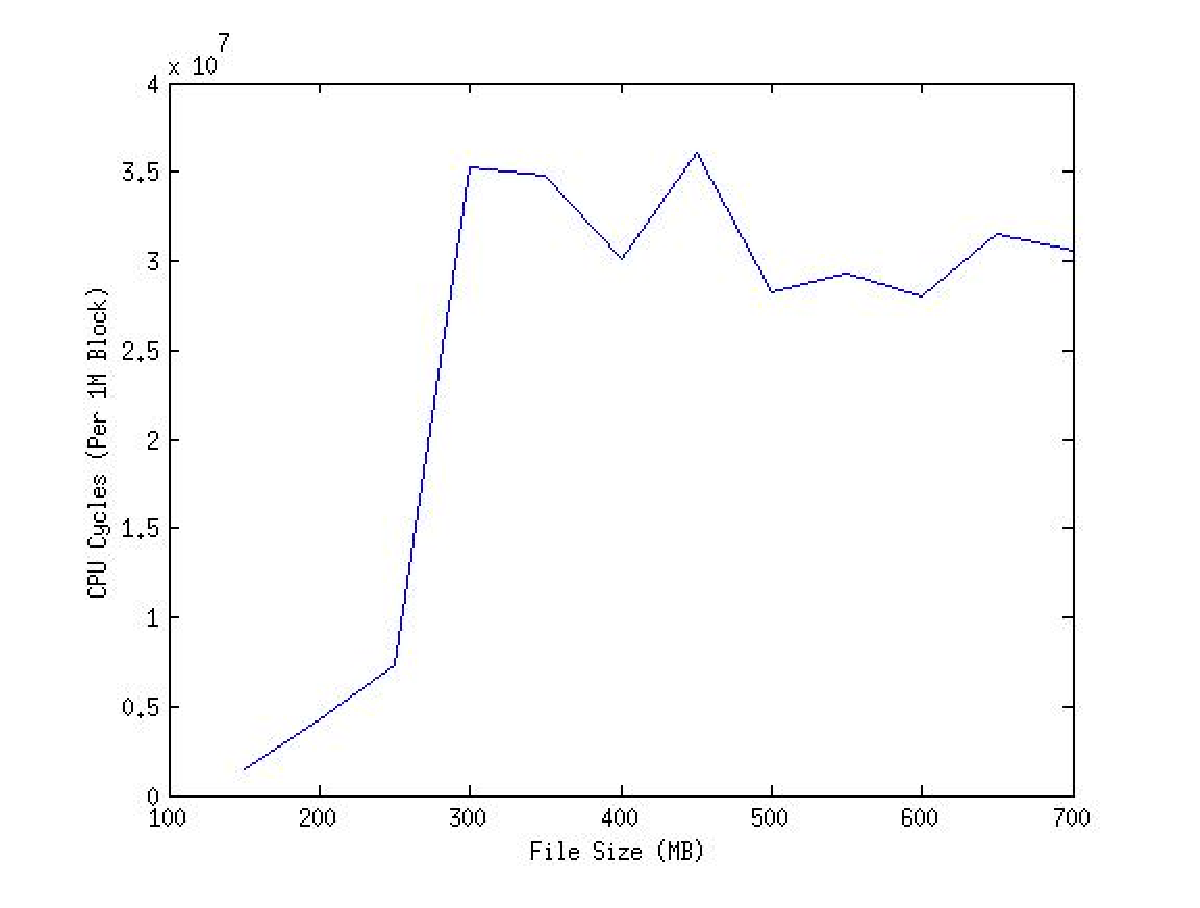
\includegraphics[scale=0.5]{res4_1}}


\subsubsection{Analyis :}

The graph clearly shows that as file size reaches 300M we see a bump
in the average read time. The RAM in our system is close to 500M,
thus file cache of 300M seems to be a pretty convincing result.


\subsection{File Read time:}


\subsubsection{Prediction}

We expect file read time to be worse for a random read when compared
to a sequential read (when we don't use file cache). This is beacuse
sequential read on disk involves less seek time.


\subsubsection{Experiment}
\begin{enumerate}
\item Open a file in O\_DIRECT mode, this ensures that no file cache is
used

\begin{enumerate}
\item Read the file sequentially, measure time 
\item Read the file randomly (using preads) and generating a random offset,
measure time 
\item Repeat (a) - (c) by increasing the size of file\end{enumerate}
\begin{lyxlist}{00.00.0000}
\item [{{%
\begin{tabular}{|c|c|c|c|c|}
\hline 
File Size(MB)  & \multirow{1}{*}{Sequential (M CPU) } & Sequential Time(ms)  & Random (M CPU)  & Random(ms)\tabularnewline
\hline 
\hline 
32  & .584  & 0.2163  & .597  & 0.2212\tabularnewline
\hline 
64  & .587  & 0.2212  & .598  & 0.2218\tabularnewline
\hline 
150  & .591  & 0.2190  & .601  & 0.2229\tabularnewline
\hline 
200  & .591  & 0.2192  & .619  & 0.2296\tabularnewline
\hline 
250  & .613  & 0.2273  & .645  & 0.2391\tabularnewline
\hline 
300  & .616  & 0.2285  & .615  & 0.2279\tabularnewline
\hline 
400  & .588  & 0.2179  & .609  & 0.2257\tabularnewline
\hline 
 &  &  &  & \tabularnewline
\end{tabular}}}] ~ 
\end{lyxlist}
\item 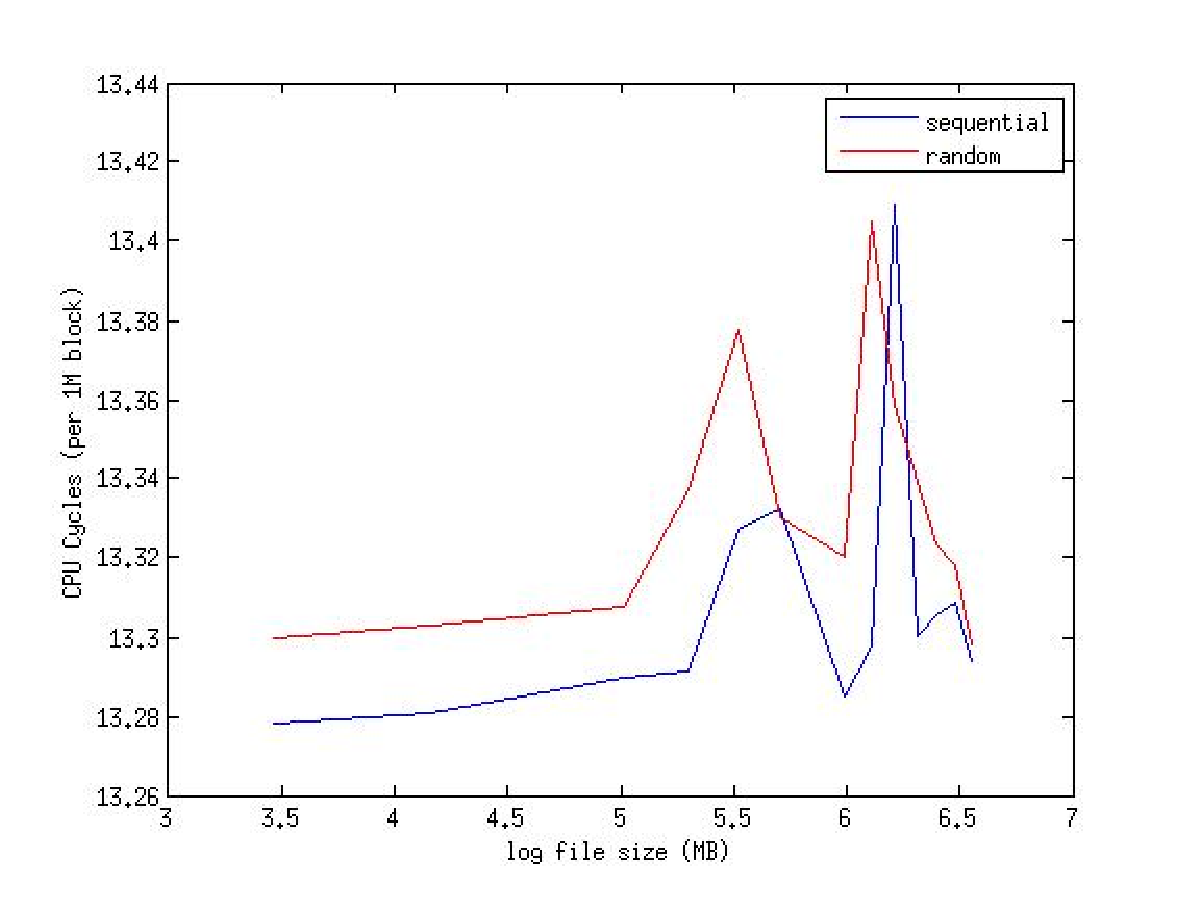
\includegraphics[scale=0.5]{res4_2} 
\end{enumerate}

\subsubsection{Analysis}

It seems from the graph that sequential writes work little bit better
than random writes.


\subsection{Remote file read time}


\subsubsection{Prediction}

Network penalty is going to overshadow any difference between sequantial
and random read. Also, we predict that network penalty is going to
be very high.


\subsubsection{Experiment}
\begin{itemize}
\item Continuing the setup of last experiment, start a nfs server and share
a folder across network 
\item Mount the shared folder on a client 
\item Read files in increasing order of size from the client, measure time
to do sequential as well as random read 
\end{itemize}

\subsubsection{Results:}

\begin{tabular}{|c|c|c|c|c|}
\hline 
File Size(MB)  & CPU Cycles - Sequential(Million)  & Time(s)  & CPU Cycles- Random (M)  & Time\tabularnewline
\hline 
\hline 
32  & 2555  & 0.9465  & 2885  & 1.0686\tabularnewline
\hline 
64  & 2456  & 0.9099  & 2617  & 0.9694\tabularnewline
\hline 
150  & 2933  & 1.0861  & 2673  & 0.9898\tabularnewline
\hline 
200  & 2830  & 1.0485  & 2816  & 1.0430\tabularnewline
\hline 
250  & 3012  & 1.1171  & 2915  & 1.0795\tabularnewline
\hline 
300  & 2569  & 0.9515  & 2837  & 1.0509\tabularnewline
\end{tabular}

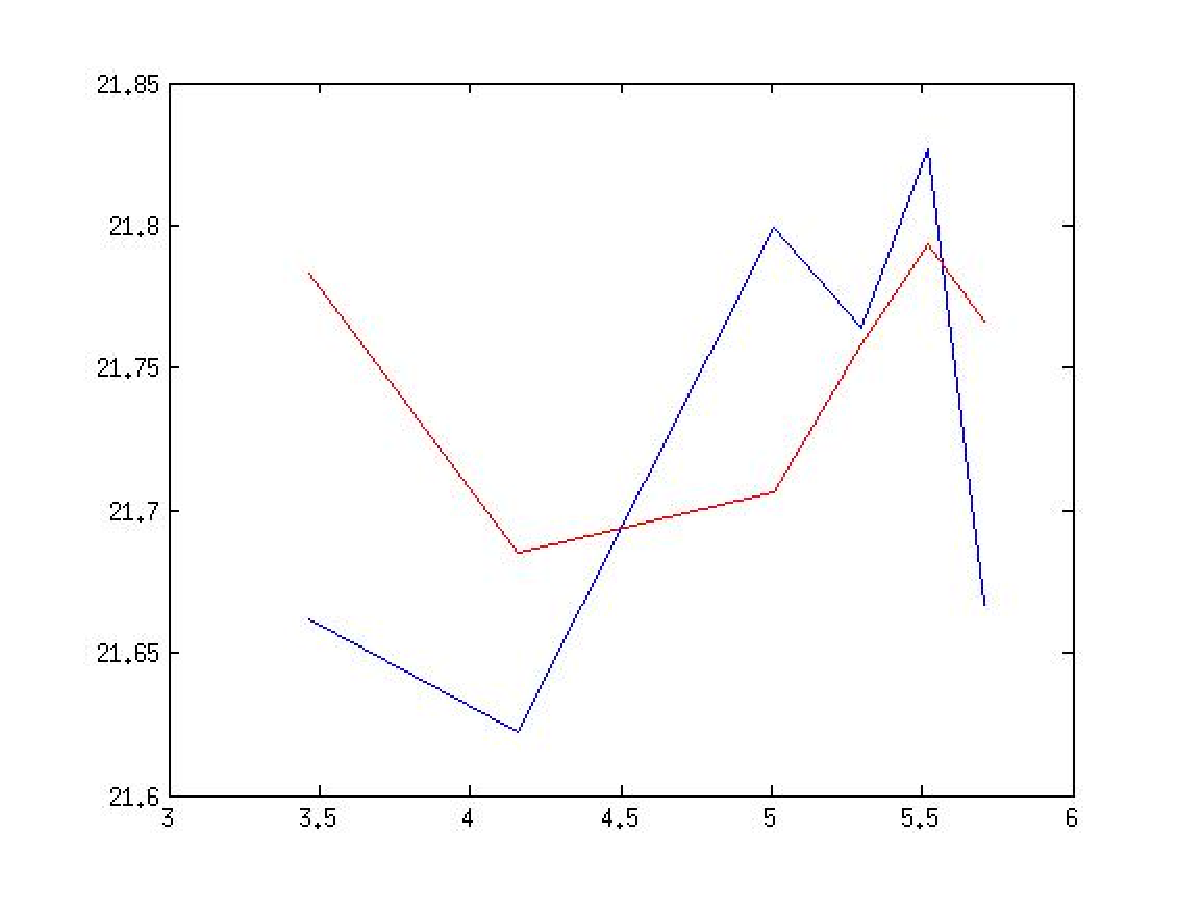
\includegraphics[scale=0.5]{res4_3}


\subsubsection{Analysis}

Network Penalty seems to be of the order of 0.8 seconds. Read time
for one block was in milliseconds, but over NFS this is in terms of
seconds. Also, its interesting to note that affect of random read
has been nullified.


\subsection{Measuring contention:}

We are measuring the effect on read operation time when number of
processes reading potentially different files in the same filesystem
(hence the same 2disk) increase.


\subsubsection{Prediction}

We expect read time to increase as number of processes in the system
(doing some read operation) increase. As number of processes increase
they will cause the disk head to move more and thus from the perspective
of one process seek time will increase - even when it is doing a sequential
access. However there might not be a direct correlation with number
of processes. All we predict is that we are going to see increase
in read time as there are other processes reading on the disk.


\subsubsection{Experiment }
\begin{itemize}
\item Set block size as 4K. Note that this does not need to be 4K, but when
measuring time per block size, we would make this block size as fixed
so that we are comparing the same quantities 
\item Create a file of 100M. Read it for a fixed number of iterations (Do
repeated reads on this file) 
\item Open all files for this experiment using O\_DIRECT. This ensures that
we are not using file cache and are directly accessing disk 
\item Measure time taken to read one block when 1 other process is reading
a file (this file is differnt than first process 
\item Measure time to read when 2 processes are reading 2 different files 
\item Continue this experiment by reading a file when 20 processes are running. 
\item Compare results 
\end{itemize}

\subsubsection{Results}

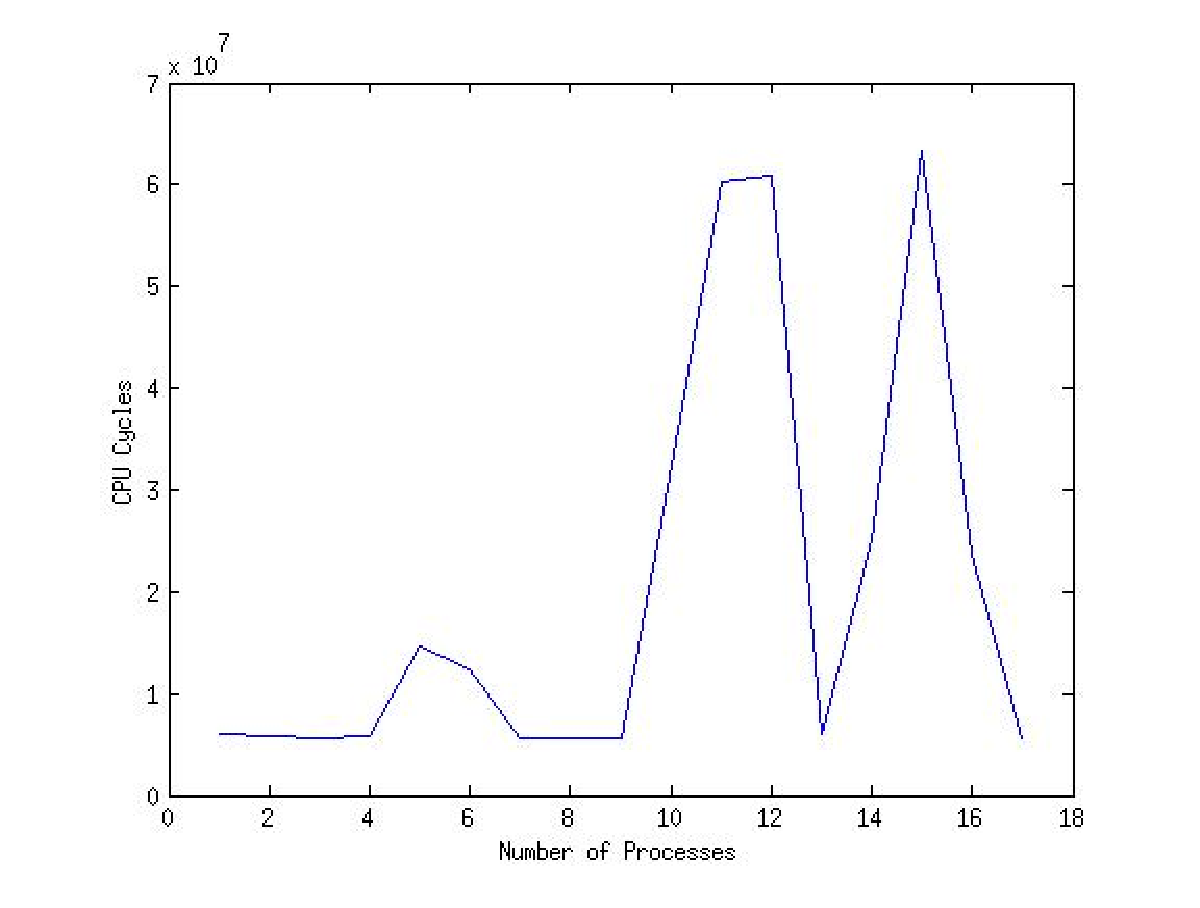
\includegraphics[scale=0.5]{res1}


\subsubsection{Analysis}

Graph shows that as number of processes increase the variations in
reading time increase too. Thus our original prediction that as more
processes try to read a file on sam disk, seek time should vary a
lot, seems correct 
\begin{thebibliography}{References}
\bibitem{key-2}Larry McVoy and Carl Staelin, lmbench: Portable Tools
for Performance Analysis, Proc. of USENIX Annual Technical Conference,
January 1996.

\bibitem{key-3}Aaron B. Brown and Margo I. Seltzer, Operating system
benchmarking in the wake of lmbench: a case study of the performance
of NetBSD on the Intel x86 architecture, Proc. of ACM SIGMETRICS,
pp. 214-224, June 1997.

\bibitem{key-5}John K. Ousterhout, Why Aren't Operating Systems Getting
Faster as Fast as Hardware?, Proc. of USENIX Summer Conference, pp.
247-256, June 1990.\end{thebibliography}

\end{document}
